\section{Anomaly detection with generative models: practical example} \label{sec:alfven}
In this section, an application of generative modelling on a practical example is presented. It was previously published in~\cite{vskvara2020detection}. Some of different generative autoencoders presented in Sec.~\ref{vae_models} will be used here to model data measured in a complex scientific experiment. Apart from the comparison of the previously presented anomaly scores, consider this to be a preliminary exploration of the already mentioned two-stage modeling principle, where an autoencoding model is used to create meaningful low-dimensional representation of complex data, and which is then coupled with some classical detector from Sec.~\ref{sec:taxonomy}. This concept will also be further explored in Chapter~\ref{sec:chapter_sgvaegan}.

\section{Chirping modes on the COMPASS tokamak}
\begin{figure}[t]%[!htbp]
  \centering
  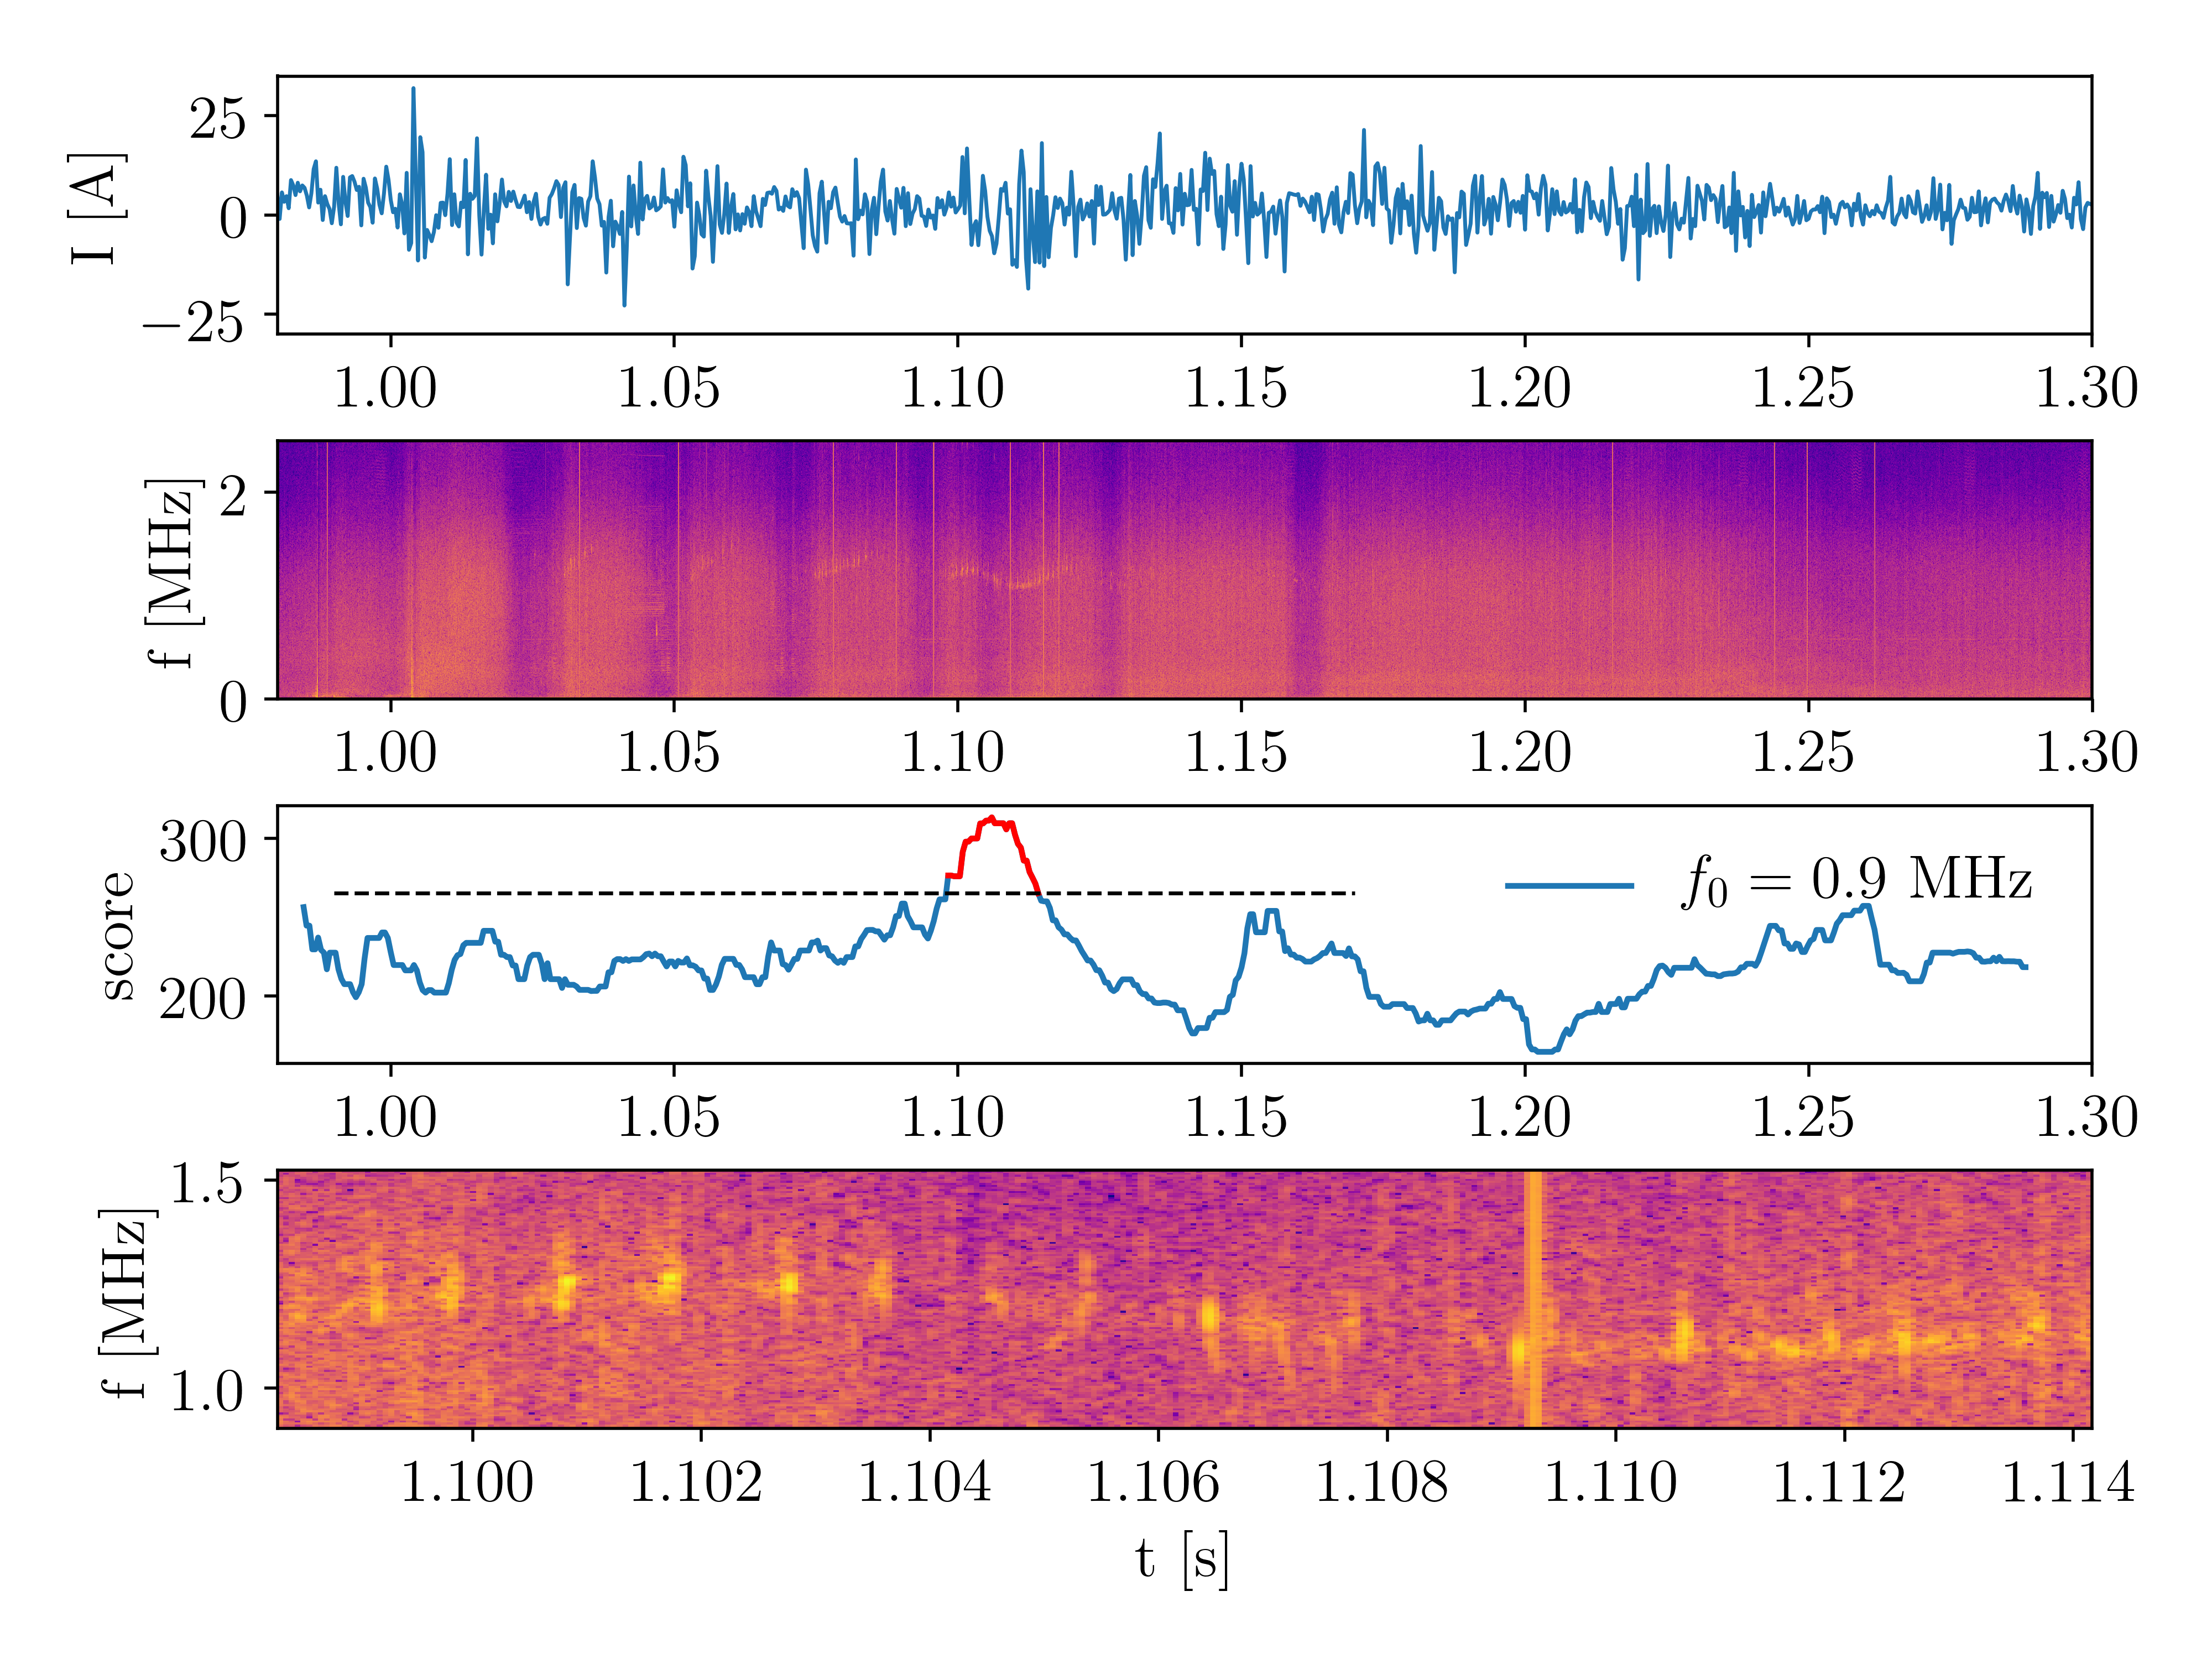
\includegraphics[scale=0.7]{data/chapter_alfven/overview.png}
  \caption{COMPASS shot 10870. Raw U-probe signal is in the upper plot. The corresponding spectrogram is below that. The score is the output of one of tested models over the spectrogram at $f_0=0.9$ MHz and it is plotted third from the top. The highest peak around 1.1s corresponds to a detected chirping mode. A close-up of the spectrogram part containing the chirping mode as detected from the red part of the score plot is at the bottom. The size of the close-up is 128 $\times$ 311 pixels.}
  \label{fig:psd}
\end{figure}

\subsection{The application problem}
As already mentioned in the introductory chapter, physics has recently enjoyed an influx of very large amounts of data~\cite{bird2011computing,ball2010data} that needs to be processed and most importantly, from which new scientific discoveries may be extracted. This is also true for the field of plasma fusion, which strives to ignite and control a fusion reaction as a clean and basically inexhaustible source of energy. The ITER project~\cite{holtkamp2007overview} is expected to produce up to 2 petabytes of data every day. This naturally calls for automatic processing of the data for a multitude of tasks, including anomaly detection. In this section, an anomaly detection problem that appears during the operation of the COMPASS~\cite{panek2015status} tokamak will be dissected.

During the operation of COMPASS, \textbf{Alfv\'en eigenmodes}~\cite{markovic2015alfven, melnikov2015quasicoherent, markovic2017alfven} were observed. Alfv\'en eigenmodes are magnetic instabilities that degrade the performance of the tokamak and possibly endanger and the plasma-facing components of the magnetic chamber~\cite{mett1992kinetic}. For this reason, their automatic detection is very important. Also, it may offer an opportunity for the study of their interactions with high-energy particles present in the plasma during an experiment. On COMPASS, chirping Alfv\'en eigenmodes are estimated to appear in about 0.1\% of all experiments. The primary means of their identification is manual inspection of spectrograms drawn from the signal of certain magnetic probes, which is very time-consuming. See Fig.~\ref{fig:psd} for an example of the measured signal, a spectrogram that is derived from it and a detected chirping Alfv\'en eigenmode. The spectrograms such as the one in Fig.~\ref{fig:psd} are large, so they are divided into patches of 128x128 pixels which is a feasible input size for current convolutional neural network architectures. It is also enough to capture most of a typical chirping mode as can be seen in the bottom plot in Fig.~\ref{fig:psd}. The patches that contain a chirping Alfv\'en eigenmodes are considered to be anomalies. There are about 200 labeled examples of patches with a chirping Alfv\'en eigenmode and a large database of unlabeled data. This is a typical anomaly detection problem, where labeled anomalies are only used for evaluation and comparison of different models and the training dataset is considered to be anomaly-free.

\subsection{The experimental setup}
Two basic experimental setups are tested in this section. Both are be based on generative autoencoders from Sec.~\ref{sec:vae_models}. The basic models have similar architectures, but they differ in the probability divergences used to regularize the latent space. The KLD~\eqref{eq:vae_kld} of a VAE model is compared against the MMD~\eqref{eq:mmd}. A WAE model with a discriminator is regularized by JSD which results in the training losses~\cite{eq:aae_loss_disc} and~\cite{eq:aae_loss_autoencoder}. Finally, a plain AE from Sec.~\ref{sec:reconstruction_models} is included to verify that a regularized latent space is useful. The individual components of the models (encoders, decoders, discriminators) are represented by neural networks with convolutional architecture. This is the most often used architecture for image data, as several levels of convolution operations are designed to capture shift invariant features at different scales of an image. For more technical details on the construction of the models, see~\cite{vskvara2020detection}. A schematic of a convolutional autoencoder is in Fig.~\ref{fig:ae}.

\begin{figure}[htpb]
\begin{center}
\begin{tikzpicture}[scale=1, transform shape]
  \vspace{-10cm}
  \node (image) at  (0,0) {\includegraphics[width=\linewidth]{data/chapter_alfven/model_structure.pdf}};
  \node (encdim) at (-4,\capy) {$\x \in \mathbb{R}^{128\times128\times1}$};
  \node (decdim) at (4,\capy) {$\hat{\x} \in \mathbb{R}^{128\times128\times1}$};
  \node (latdim) at (0, \capy) {$\z \in \mathbb{R}^{d}$};
  \node (enc) [align=left] at (\encx, .5) {encoder\\ $e_{\phi}(\x)$};%{$e_{\phi}(\x)$};
  \node (enc) [align=left] at (\encx, -.5) {Conv. +\\ Dense};
  \node (dec) [align=left] at (\decx, .5) {decoder\\ $d_{\theta}(\z)$};%{$d_{\theta}(\z)$};
  \node (dec) [align=left] at (\decx, -.5) {Dense +\\ Tr. Conv.};
\end{tikzpicture}
\end{center}
\caption{A schematic diagram of the convolutional autoencoder used for our experiments. Spectrogram patches are encoded through several convolutional\cite{lecun1989backpropagation}, maxpooling\cite{ranzato2007efficient} and dense (fully connected) layers into $d$-dimensional vectors (here $d=2$) and then decoded back with transposed convolutions and upscaling layers.}
\label{fig:ae}
\end{figure}

In the first setup, the described models are compared against each other as primary anomaly detectors. This means that they are trained on the (assumed) normal spectrogram patches and the anomaly scores derived in their respective sections are 


\subsection{One-class model}
In the first model, we will use a convolutional generative autoencoder as a one-class estimator. This is an approach well known in the anomaly/outlier detection setting\cite{chandola2009anomaly,scholkopf2001estimating}. A model of choice learns a representation of one class of data and can, therefore, be used to detect out-of-class samples. It is trained either with labeled data belonging to the class of interest, or with unlabeled data which are believed to contain so little out-of-class examples that the model is robust enough to ignore them. 

A generative autoencoder can be readily used for this task if we set $p_{\theta}(x) \approx p(x)$ to be the distribution of the class of our interest. Then there are two modes of training the autoencoder. In the first mode, we model the distribution of patches that contain a chirping mode. Then the autoencoder is trained with the positively labeled data. However, this is a bit problematic since there are very few labeled patches available, therefore the neural network will very likely overfit. In the second mode, we can choose the class of interest to be of the patches that do not contain a chirping mode. This is closer to an anomaly detection formulation of the problem, as the relatively rare chirping modes are considered to be anomalous. Also, the autoencoder can be trained with unlabeled data due to the sparse occurrence of chirping modes and robustness of probabilistic neural networks\cite{an2015variational,leveau2017adversarial}, hugely increasing the number of training samples and thus the representative power of the neural network. On the other hand, this might

To decide whether a sample $x$ is in- or out-of-class, we can compute its negative loglikelihood under the generative distribution 
\begin{equation} \label{eq:llh}
  -\mathbb{E}_{q_{\phi}(z|x)}\left[\ln p_{\theta}(x|z)\right]
\end{equation}
or its approximation, the MSE between $x$ and its (sampled) reconstruction $\hat{x}$. In our experiments, we use loglikelihood~\eqref{eq:llh} since it better captures the uncertainty in the reconstruction.

\subsection{Two-stage model}
The second model is designed to make the most use of both labeled and unlabeled data. It exploits the ability of generative autoencoders to produce low dimensional uncorrelated representation of high dimensional image data. It consists of two stages. The first stage is a convolutional generative autoencoder trained with unlabeled data. Its task is to learn the general topology of the input space and encode input data. The second stage is a classifier that is trained on encoded labeled data. Through the use of MMD or $\text{JS}_D$ measures and VampPrior, we can enforce separation of the encoded data into clusters that contain similar inputs, which makes the task of the classifier easier. Two different classifiers were tested.


\paragraph{kNN} The kNN algorithm for classification\cite{deng2016efficient} was trained using the labeled training data. In this setting, an unlabeled sample is given a score based on the average label of its $k$-nearest neighbors. The more neighboring training samples are labeled as positive, the higher the score.

\paragraph{GMM} A Gaussian Mixture Model (GMM)\cite{huang2005gaussian} with $M$ components was fitted on the latent representations of both labeled and unlabeled training data. Afterward, we determine one or more components of the mixture into which the positively labeled training samples are most likely to be projected via the encoder. Then, for a new sample, the score is the (average) loglikelihood of the sample in the anomalous components. 

\subsection{Experimental setup}

\subsection{Data}
Every spectrogram was divided into patches of size $128\times128$ pixels. Out of 40 pre-processed spectrograms, 370 non-overlaping patches were extracted and labeled. This results in a labeled training dataset $\left\{ X_{l},Y\right\} ,X_{l}=\left\{ x_{i}\right\} _{i},x_{i} \in \mathbb{R}^{128\times128\times1}, Y=\left\{ y_{i}\right\} ,y_{i}\in\left\{ 0,1\right\}$ of samples $X_{l}$ and labels $Y$, where $Y=1$ if a patch contains a chirping mode. Also, an unlabeled database $X_{u}$ of 330000 patches coming from 2000 spectrograms was created. 

Training of the one-class model was done both with labeled positive spectrograms and on the large unlabeled dataset. In the first case, the 50\% of positive spectrograms were used for training and the rest together with the unlabeled ones for testing. Also, training patches were randomly shifted and noise was added to them so that there were a total of $10^4$ training samples. In the second case, all of the labeled data was only used for testing. 10 different training and testing datasets were created this way for cross-validation purposes.

For training of the two-stage model, we have split the labeled dataset to training/testing subsets with the ratio 80/20. Again, this splitting was done randomly a total of 10 times.

\subsection{Model architecture and hyperparameters}

\begin{table}
\centering

\captionsetup[subtable]{position = below}
\captionsetup[table]{position=below}

\begin{subtable}{0.4\linewidth}
  \centering
  \begin{tabular}{c | c}
     parameter & values\tabularnewline
    \hline 
    $\gamma$ & $\left\{ 10^{0},10^{-1},10^{-2}\right\} $\tabularnewline
    $\lambda,\lambda_{1},\lambda_{2}$ & $\left\{ 10^{1},10^{0},10^{-1}\right\} $\tabularnewline
    $d$ & $\left\{ 8, 128,256\right\} $\tabularnewline
    
  \end{tabular}
  \caption{One-class model.}
  \label{tab:1c_params}
\end{subtable}
\hspace*{4em}
\begin{subtable}{0.4\linewidth}
  \centering
  \begin{tabular}{c  c | c}
      & parameter & values\tabularnewline
    \hline 
    \multirow{4}{*}{1st stage} & $N$ & $\left\{ 1,2,4,8\right\} $\tabularnewline
    & $\gamma$ & $\left\{ 10^{0},10^{-1},10^{-2}\right\} $\tabularnewline
    & $\lambda,\lambda_{1},\lambda_{2}$ & $\left\{ 10^{1},10^{0},10^{-1}\right\} $\tabularnewline
    & $d$ & $\left\{ 2,16,32,64\right\} $\tabularnewline
    \hline
    \multirow{2}{*}{2nd stage} & $k$ & $\left\{ 1,3,\ldots,31\right\} $\tabularnewline
    & $M$ & $\left\{ 2,4,6,8\right\} $\tabularnewline

  \end{tabular}
  \caption{Two-stage model.}
  \label{tab:2s_params}
\end{subtable}
\caption{Overview of model hyperparameters. $\lambda_{1}$ and $\lambda_{2}$ are scaling parameters for the combination of MMD and adversarial loss.}
\end{table}

\paragraph{One-class model}
The architecture for the one-class encoder was 2 or 3 convolutional layers with (32,64) or (32,32,64) channels and kernel size of 5. Each convolutional layer was followed by a maxpooling layer which downscaled the image by a factor of 2. Then a dense layer produced the final encoding into a $d$-dimensional latent space. The decoder mirrored the encoder architecture with transposed convolutions in place of maxpooling layers. ResNet\cite{he2016deep} type residual blocks were used to speed up and stabilize the training. The hyperparameter values over which we have optimized trained models are in Tab.~\ref{tab:1c_params}.
Parameter $\gamma$ denotes the scaling parameter of the inverse multiquadratics (IMQ) kernel\cite{gorham2017measuring}.

\paragraph{Two-stage model}
The basic encoder architecture was the following: 3 convolutional layers with (16,16,32) channels and kernel size of 3, (2,2,1) downscaling ratios via maxpooling, followed by two dense layers of width (256,$d$) where $d$ is the dimension of the latent space. The decoder mirrored this architecture. Also, batch normalization\cite{ioffe2015batch} was used. The hyperparameter values over which we have optimized are in Tab.~\ref{tab:2s_params}. The number of components in the used prior is denoted by $N$. 

The base architecture of the two models is slightly different. We have experimented with different architectures prior to the hyperparameter optimization and found that for the different tasks, different architectures provide better results. This is probably due to the fact that both models have a different objective - the one-class model requires precise reconstruction, while the two-stage is evaluated based on the shape of latent space. Ideally, we would include architectures as a tunable parameter, but that would require a level of computational power that was not available to us.

Both models use ReLu\cite{hahnloser2000digital} activation and were optimised with the RMSProp optimizer with learning rate $10^{-4}$. For a single optimization iteration, batches of 128 patches were used. We have implemented all the models in the Julia language\cite{bezanson2017julia} and trained them on TITAN V Nvidia GPU with 12 GB of memory. 

\section{Results}

In this section, the result of experiments with one-class and two-stage models are going to be examined and compared. Also, we will discuss the importance of an appropriate train/test splitting strategy that was used in our experiments in order not to obtain overly optimistic model performance estimates.

\subsection{Output evaluation}

\begin{figure}
\begin{centering}
\includegraphics[scale=0.5]{data/chapter_alfven/anomalies.png}
\par
\end{centering}
\caption{Examples of spectrogram patches identified as containing a chirping
mode.}
\label{fig:alfven_patches}
\end{figure}

In case our framework was implemented in a production environment, the working scenario would be the following. A set of experiments to be analyzed would be selected. Then, the needed signals would be extracted, spectrograms computed and divided into patches of appropriate size. These would be fed to a trained model that would produce scores to enable ranking of the patches. Since this would produce hundreds, maybe thousands of patches and scores, the operator would ideally only want to go through a few with the highest score. In Fig.~\ref{fig:alfven_patches} we show the output of such procedure --- 4 patches with the highest score, out of which 3 contain a chirping mode. It illustrates that even though the neural network encoding might be powerful, it is still basically a black box model and we need to be very careful in its evaluation. Because of this, we evaluate the model performance by computing AUC (area under the receiver operating curve), which is a standard measure for binary classification problems, and also by precision@$k$ score, which is the precision at the $k$-highest scoring samples. 

\subsection{One-class model optimization}

\begin{table}
  \centering
  \begin{tabular}[h]{c c c c} 
divergence & target class & AUC & precision@50 \\ 
\hline 
-- & Alfv\'en & $0.57 \pm 0.04$ & 0.24 $\pm$ 0.05 \\ 
KLD & Alfv\'en & 0.74 $\pm$ 0.06 & 0.44 $\pm$ 0.13 \\ 
MMD & Alfv\'en & 0.77 $\pm$ 0.03 & 0.49 $\pm$ 0.06 \\ 
JSD & Alfv\'en & 0.69 $\pm$ 0.07 & 0.42 $\pm$ 0.08 \\ 
MMD + JSD & Alfv\'en & 0.72 $\pm$ 0.09 & 0.37 $\pm$ 0.03 \\
-- & non--Alfv\'en & 0.82 $\pm$ 0.03 & 0.86 $\pm$ 0.06 \\ 
KLD & non--Alfv\'en & 0.46 $\pm$ 0.05 & 0.50 $\pm$ 0.14 \\ 
MMD & non--Alfv\'en & 0.84 $\pm$ 0.03 & \textbf{0.90 $\pm$ 0.06} \\ 
JSD & non--Alfv\'en & 0.84 $\pm$ 0.05 & 0.83 $\pm$ 0.10 \\ 
MMD + JSD & non--Alfv\'en & \textbf{0.84 $\pm$ 0.01} & 0.87 $\pm$ 0.01 \\ 
\end{tabular}

  \caption{Results of optimization of the one-class model. Target class differences are described in the experimental setup section. No divergence is a plain autoencoder with MSE training objective.}
  \label{tab:one_class}
\end{table}

The hyperparameter optimization routine resulted in hundreds of trained models. To select the best one, the AUC and precision@50 measures were computed on a testing dataset. Then, for a set of fixed hyperparameter values, these were averaged over 10 cross-validation test-train splits. The best results for a combination of target class and used divergence based on these measures are reported in Tab.~\ref{tab:one_class}. Clearly, it seems that modeling the distribution of chirping mode spectrograms is more difficult than vice versa with the exception of KLD, which completely fails. Also, the precision in top samples is very low in the Alfv\'en target class. Surprisingly, a plain autoencoder achieves results almost comparable to other models. In Fig.~\ref{fig:roc_prc} are the ROC (receiver operating characteristic)\cite{fawcett2006introduction} and PR (precision-recall)\cite{boyd2013area} curves of the single best performing one-class models as well as the two-stage models.

\begin{figure}
\begin{centering}
\includegraphics[scale=0.6]{data/chapter_alfven/roc_prc.pdf}
\end{centering}
\caption{ROC and PR curves of selected models.}
\label{fig:roc_prc}
\end{figure}

\subsection{Two-stage model}

\begin{table}
\centering
\begin{tabular}{c c c c}
	\toprule
	divergence & classifier & AUC & precision@50  \\
	\midrule
	-- & kNN & 0.80$\pm$0.07 &  \cellcolor{gray!15} 0.88$\pm$0.10 \\
	KLD & kNN & 0.80$\pm$0.08 & 0.85$\pm$0.11 \\
	MMD & kNN &  \cellcolor{gray!45} 0.91$\pm$0.06 &  \cellcolor{gray!45} 0.94$\pm$0.05\\
    JSD & kNN &  \cellcolor{gray!15} 0.83$\pm$0.07 & 0.87$\pm$0.10\\
    MMD + JSD & kNN &  \cellcolor{gray!30} 0.86 $\pm$ 0.07 &  \cellcolor{gray!30} 0.91$\pm$0.10 \\
    -- & GMM & 0.75$\pm$0.06 & 0.80$\pm$0.10\\
	KLD & GMM & 0.74$\pm$0.06 & 0.83$\pm$0.11\\
	MMD & GMM & 0.66$\pm$0.12 & 0.72$\pm$0.12\\
    JSD & GMM & 0.74$\pm$0.06 & 0.82$\pm$0.11\\
    MMD + JSD & GMM & 0.76$\pm$0.06 & 0.84$\pm$0.10 \\
    \bottomrule
\end{tabular}
\caption{Results of hyperparameter tuning of the two-stage model across 10 cross-validation splits.}
\label{tab:alfven_results}
\end{table}

Here, we evaluate the performance of the two-stage model. The methodology of hyperparameter optimization via cross-validation is similar to that used for the one-class model.  The best average result across 10 splits for different combinations of stage one divergences and stage two classifiers are reported in Tab.~\ref{tab:alfven_results}. The simple kNN model is superior to the GMM approach. Also, MMD regularization seems to produce the best results. We might speculate that this might be due to the improved ability to produce a well-separated encoding enforced by the used prior. Again, in Fig.~\ref{fig:roc_prc} see the ROC and PRC curves for the single best two-stage models.

A question one might ask is whether the autoencoding is truly necessary. In the end, we are doing a projection from $d=128\times128=16384$ dimensional picture space into at most $d=64$ dimensional latent space which must naturally lead to a loss of information. As shown in Fig.~\ref{fig:patches_latent}, where $d=8$, the autoencoder is able to identify the difficult nonlinear correlations and improve the performance of a subsequent second stage kNN model. The compression is clearly necessary for overcoming the curse of dimensionality which implies that L$_2$ distance degenerates in large dimensions. An alternative approach to overcoming the issue of large input dimension might be to train a classification convolutional neural network, which does the compression by its nature. We have not chosen to go this path however since we believe that such a network would be highly susceptible to overfitting since it requires a lo of labeled data which is not available to us. Instead, we have tried to overcome this in the two-stage model by learning the compression from all the available unlabeled data.

\subsection{Influence of the train/test splitting methodology}

\begin{figure}
\centering
\includegraphics[scale=0.45]{data/chapter_alfven/split_patches.pdf}
\includegraphics[scale=0.45]{data/chapter_alfven/split_spectrograms.pdf}
\caption{kNN fits for different values of $k$. The red line and band show the mean and one standard deviation bands of the resulting AUC values when kNN is fitted to the original vectorized images. The input space dimensionality is $d=16384$. The blue dashed line and band are the same quantities for a $d=8$ dimensional representation by a first stage model. On the left, the training and testing splits were done on the level of individual patches, leading to a better performance and less variance. On the right, the split was done on the level of the original spectrograms, which is a more realistic scenario. The standard deviation and mean were computed from 10 random splits.}
\label{fig:patches_latent}
\end{figure}

At first, the splitting of testing and training labeled patches was done on the level of patches, without any regard for the spectrogram/experiment that the patch came from. It was assumed that the labeled chirping modes are homogeneous across the spectrograms. However, this turned out not to be true. Therefore, the train/test splits were done on the level of spectrograms which were then subsequently divided into patches. See Fig.~\ref{fig:patches_latent} where on the left side, the AUC curves for different values of $k$ of the kNN model are for the case when the data split was done on the level of patches. The blue line that is the result of kNN fit peaks at $k=3$. On the other hand, there is no such peak on the right side of the figure, where splitting was done on the level of spectrograms. This indicates that the positively labeled patches in a single spectrogram are much more similar to each other than to those in different spectrograms, as only a relatively low number of neighbors is sufficient for optimal performance. Also, the variance of the right side plots is much higher, again indicating larger differences across spectrograms. If we continued with the splitting on the level of patches, we would have a biased and too optimistic estimate of performance before putting the framework into production.

\section{Conclusion}
Our task was identification of anomalous phenomena --- chirping Alfv\'en modes --- in graphical representations of signals measured during the operation of a tokamak. To this end, we have proposed two models based on generative autoencoders. The first model learned the distribution of normal data and identified chirping modes as out-of-class samples of this distribution. The second model implemented a two-stage learning approach. A regularized convolutional variational autoencoder trained on unlabeled data was successfully combined with a classifier trained with a smaller labeled dataset. It has been shown that both models are viable options in chirping mode identification, although the latter one proved to be superior.

We have also shown the need for proper cross-validation splitting of data in the evaluation phase and outlined the need for careful evaluation in order for the model to be useful in real-world application. However, this is still work in progress. We mentioned the need to use a more appropriate evaluation measure that reflects the operational conditions. Furthermore, so far we have only used spectrograms from a single U probe, but there are about 40 more magnetic diagnostics that could be potentially used for this task, e.g. their spectrograms/correlograms could be added as an additional input channel. Finally, a more thorough evaluation of the contemporary experimental results is needed for the understanding of the framework behavior and to be applicable to COMPASS operation, most likely through the expansion of the labeled dataset. 
